\documentclass[tikz,border=10pt]{standalone}
\usepackage{tikz}
\usetikzlibrary{arrows.meta,decorations.pathreplacing,calc,patterns}

\definecolor{ink}{HTML}{363636}
\definecolor{xred}{HTML}{CC2E40}     % X axis
\definecolor{ygreen}{HTML}{2E7D32}   % Y axis  (clearer green for "out/in of page")
\definecolor{zblue}{HTML}{1F4E9F}    % Z axis

\begin{document}
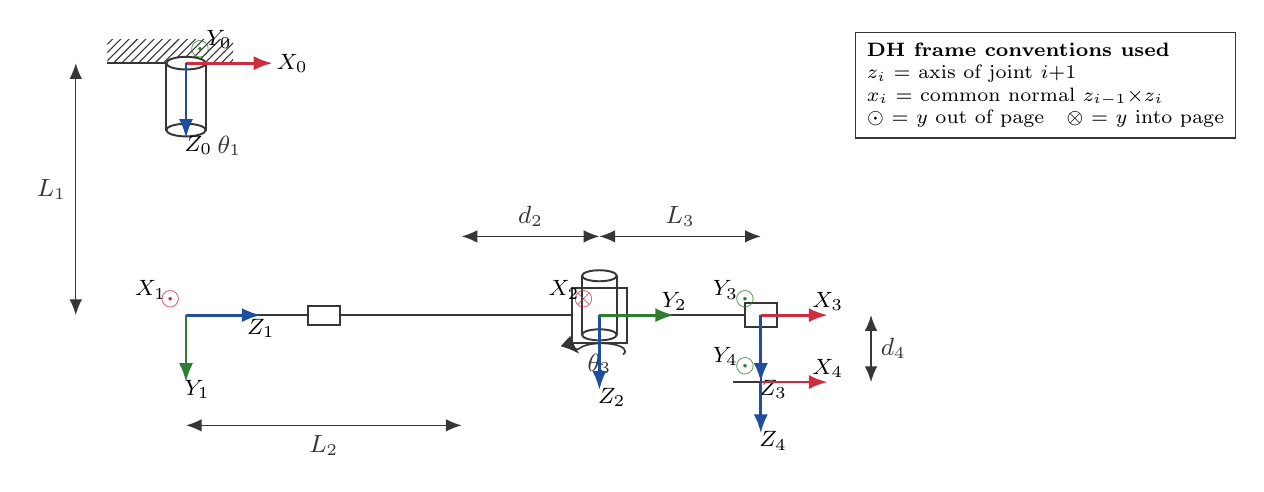
\begin{tikzpicture}[
    >={Latex[length=2.4mm,width=1.8mm]},
    line cap=butt, line join=miter,
    every node/.style={font=\small},
    link/.style={ink, line width=0.9pt},
    axis/.style={line width=1.0pt},
    dim/.style={ink, line width=0.5pt, <->, >={Latex[length=2mm,width=1.6mm]}},
    joint/.style={ink, fill=white, line width=0.7pt},
    flbl/.style={font=\footnotesize, inner sep=1pt},
]

% ============================================================
% Geometry constants
% ============================================================
\def\Lone{3.2}
\def\Ltwo{3.5}
\def\Dtwo{1.75}
\def\Lthree{2.05}
\def\Dfour{0.85}

\coordinate (O0)    at (0, 5.4);
\coordinate (Elbow) at (0, 5.4 - \Lone);
\coordinate (J3)    at (\Ltwo + \Dtwo, 5.4 - \Lone);
\coordinate (J4)    at (\Ltwo + \Dtwo + \Lthree, 5.4 - \Lone);
\coordinate (EE)    at (\Ltwo + \Dtwo + \Lthree, 5.4 - \Lone - \Dfour);

% Ceiling + base cylinder
\fill[pattern=north east lines, pattern color=ink] (-1.0,5.4) rectangle (0.6,5.7);
\draw[ink, line width=0.6pt] (-1.0,5.4) -- (0.6,5.4);
\draw[joint] (-0.25,4.55) rectangle (0.25,5.4);
\draw[joint] (0,5.4) ellipse (0.25 and 0.08);
\draw[joint] (0,4.55) ellipse (0.25 and 0.08);

% Links
\draw[link] (Elbow) -- (O0 |- Elbow);
\draw[link] (Elbow) -- (J3);
\draw[link] (J3)    -- (J4);
\draw[joint] (1.55, 5.4 - \Lone - 0.12) rectangle (1.95, 5.4 - \Lone + 0.12);

% Joint 3 cylinder
\draw[joint] ($(J3)+(-0.35,-0.35)$) rectangle ($(J3)+(0.35,0.35)$);
\draw[joint] ($(J3)+(0,0.5)$)  ellipse (0.22 and 0.07);
\draw[joint] ($(J3)+(-0.22,0.5)$) -- ($(J3)+(-0.22,-0.25)$);
\draw[joint] ($(J3)+(0.22,0.5)$)  -- ($(J3)+(0.22,-0.25)$);
\draw[joint] ($(J3)+(0,-0.25)$) ellipse (0.22 and 0.07);

% End-effector mount + d4 + plate
\draw[joint] ($(J4)+(-0.20,-0.15)$) rectangle ($(J4)+(0.20,0.15)$);
\draw[link] (J4) -- (EE);
\draw[link] ($(EE)+(-0.35,0)$) -- ($(EE)+(0.35,0)$);

% Length dimensions
\draw[dim] (-1.4,5.4) -- (-1.4, 5.4 - \Lone) node[midway,left] {$L_1$};
\draw[dim] (0, 5.4 - \Lone - 1.4) -- (\Ltwo, 5.4 - \Lone - 1.4) node[midway,below] {$L_2$};
\draw[dim] (\Ltwo, 5.4 - \Lone + 1.0) -- (\Ltwo + \Dtwo, 5.4 - \Lone + 1.0) node[midway,above] {$d_2$};
\draw[dim] (\Ltwo + \Dtwo, 5.4 - \Lone + 1.0) -- (\Ltwo + \Dtwo + \Lthree, 5.4 - \Lone + 1.0) node[midway,above] {$L_3$};
\draw[dim] ($(EE)+(1.4,0)$) -- ($(J4)+(1.4,0)$) node[midway,right] {$d_4$};

% Theta indicators
\node[ink] at (0.55, 4.35) {$\theta_1$};
\node[ink] at ($(J3)+(0.0,-0.62)$) {$\theta_3$};
\draw[ink, line width=0.6pt, ->] ($(J3)+(0.30,-0.50)$) arc (-25:200:0.30 and 0.10);

% ============================================================
% DH frames.  Convention (Spong/standard DH):
%   z_i along axis of joint (i+1).
%   x_i along common normal of z_{i-1}, z_i (=> z_{i-1} x z_i / |..|).
%   "+" green dot = +y out of page;  "x" green crossed-circle = +y into page.
% Each frame drawn AT the configuration shown (theta1 = theta3 = 0 visually).
% ============================================================

% --- Frame {0}: given. x0 right, z0 down, y0 out of page.
\draw[axis,xred,->]  (O0) -- ++(1.1,0)   node[flbl,right,black] {$X_0$};
\draw[axis,zblue,->] (O0) -- ++(0,-0.95) node[flbl,below right=-2pt,black] {$Z_0$};
\node[ygreen] at ($(O0)+(0.18,0.18)$) {$\odot$};
\node[flbl,black] at ($(O0)+(0.42,0.30)$) {$Y_0$};

% --- Frame {1}: at elbow.  z1 along d2 axis (right).  x1 = z0 x z1 = out of page.
%     y1 = z1 x x1 = down.
\coordinate (F1) at ($(Elbow)+(0.18,0.18)$);
\draw[axis,zblue,->] (Elbow) -- ++(0.95,0)   node[flbl,below,black] {$Z_1$};
\draw[axis,ygreen,->] (Elbow) -- ++(0,-0.85) node[flbl,below right=-2pt,black] {$Y_1$};
\node[xred] at ($(Elbow)+(-0.20,0.20)$) {$\odot$};
\node[flbl,black] at ($(Elbow)+(-0.45,0.32)$) {$X_1$};

% --- Frame {2}: at J3.  z2 down (axis of theta3, chosen down so alpha3=0).
%     x2 = z1 x z2 = into page.   y2 = z2 x x2 = right.
\draw[axis,zblue,->]  (J3) -- ++(0,-0.95)  node[flbl,below right=-2pt,black] {$Z_2$};
\draw[axis,ygreen,->] (J3) -- ++(0.95,0)   node[flbl,above,black] {$Y_2$};
\node[xred] at ($(J3)+(-0.20,0.20)$) {$\otimes$};
\node[flbl,black] at ($(J3)+(-0.45,0.32)$) {$X_2$};

% --- Frame {3}: at J4.  z3 down (along d4).  z2||z3, choose x3 along L3 (right).
%     y3 = z3 x x3 = out of page.
\draw[axis,xred,->]  (J4) -- ++(0.85,0)   node[flbl,above,black] {$X_3$};
\draw[axis,zblue,->] (J4) -- ++(0,-0.85)  node[flbl,below right=-2pt,black] {$Z_3$};
\node[ygreen] at ($(J4)+(-0.20,0.20)$) {$\odot$};
\node[flbl,black] at ($(J4)+(-0.45,0.32)$) {$Y_3$};

% --- Frame {4}: end effector.  Same orientation as {3}, translated by d4 along z3.
\draw[axis,xred,->]  (EE) -- ++(0.85,0)   node[flbl,above,black] {$X_4$};
\draw[axis,zblue,->] (EE) -- ++(0,-0.65)  node[flbl,below right=-2pt,black] {$Z_4$};
\node[ygreen] at ($(EE)+(-0.20,0.20)$) {$\odot$};
\node[flbl,black] at ($(EE)+(-0.45,0.32)$) {$Y_4$};

% Legend
\node[align=left, anchor=north west, font=\scriptsize, inner sep=4pt,
      draw=ink, line width=0.4pt, fill=white]
  at (8.5, 5.8) {%
    \textbf{DH frame conventions used}\\
    $z_i$ = axis of joint $i{+}1$\\
    $x_i$ = common normal $z_{i-1}{\times}z_i$\\
    $\odot$ = $y$ out of page\quad $\otimes$ = $y$ into page};

\end{tikzpicture}
\end{document}
